\chapter{State Of Art}\label{chap:stateOfTheArt}

\minitoc


\section{Cameras positioning }\label{sec:camerasPositioning}
An efficient cameras positioning is a bottleneck in many application, as for example in the video surveillance field \cite{11*herrera2012,12*soto2009,18*ding2012,151*zhao2013,84*xu2011}. Where an efficient cameras positing is essential to monitor correctly an area.  
In the following section the question of: 
What is a good position and orientation for a camera inside the video surveillance network?
What are the objectives of the cameras positioning?
Is investigated and  some answer to this questions is proposed by an overview of the literatures, the different formulations and solutions. 


\subsection{What is an efficient pose in a camera network.}
The pose of the cameras,  is composed by the position inside the area to monitor and the orientations of it. The orientation is also called looking direction.\\ 
%An efficient pose and in some case the orientation (or also called looking direction) is directly related then the objective.\\
To evaluate if a camera  pose is efficient, it is primordial to identify the objectives. The objective is different from the finality. The objectives are the most important elements to take in consideration in order to place the set of cameras. When the finality is the global application, as for example video surveillance is the finality but the coverage of an area and a target tracking  is required to have an efficient surveillance.  The coverage is one of the objectives the most interesting and the most common has many problems about cameras positioning (It will be studied in details later).

%The coverage can be applied on cover each side of an object (as  in [142*]). But in most of the case the coverage is applied on area ( inside or outside). 

To have a clever and efficient cameras positioning system different aspects must be studied. To pose efficiently a set of cameras it is useful to know what does it mean efficient  for  the  camera pose. To do that the objective of the cameras network have to be defined clearly. 

The objective can vary and depend on the objective the camera will be affected.
The positioning of the camera is impacted by the final objective as for example; the camera will be placed differently for tag detection \cite{22*zhao2008}, then for monitoring a vast outside area \cite{146*li2011}.  In Zhao et al \cite{22*zhao2008} the camera are placed at a fixed elevation (at the height of the torso) with a looking  direction almost parallel to the ground, instead to can do the tag detection and localization with no too much deformation of the tag. Otherwise in Li et al \cite{146*li2011} an UAV is used to monitor a vast area. The camera looking direction is almost perpendicular to the ground. These 2 articles are focused on having the best coverage as possible of an area but the constraint (camera are mounted on UAV, fixed elevation and others), and the secondary objective (coverage of an area for tag detection, or cover a vast area) give to different formulation and pose estimation.
\\
The following section is focused on the cameras positioning for maximizing the viewing areas. The viewing area or the coverage rate of the area is directly linked to the pose estimation of each camera and their orientation. To have the best coverage is primordial find the best position for each cameras, depending on the constraint and the eventual secondary objectives.\\
Indeed to maximize the coverage rate by optimizing the cameras position has been developed this past decade, using many different approaches. \\
His approach is applicable depending on the formulation of the constraints and objectives. In numerous cases the maximization of the coverage is only the first part of the problem, hence the importance of secondary objectives.\\
The following part is focused on what kind of area is covered what is exactly called coverage and with the secondary objectives associated too.

\subsection{First objective : Coverage }

The coverage is the main objective but is not the finality. An efficient coverage is an requirement for many application ( video surveillance  for example) 

The focus of this study is to find the best position of each camera in order to maximize the covered area. To do that, it is important to define what is exactly mean "covered". Based on the literature the covered area can be varied, depending on the finality. 
% Among the huge possible definition more or less restrictive the more interesting to studied is discussed: 
\begin{figure}[t!]
\minipage{0.85\textwidth}
   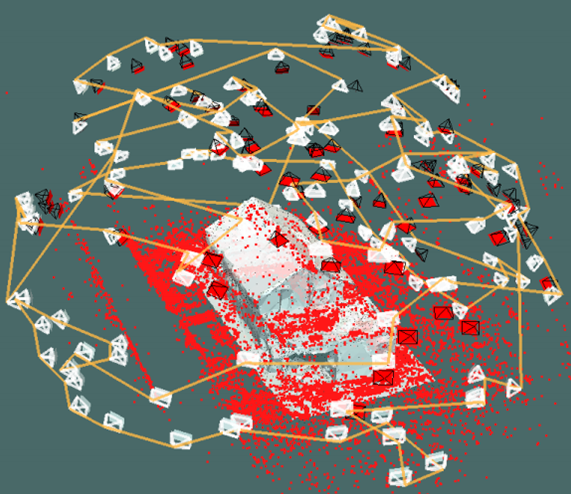
\includegraphics[width=\linewidth]{img/objectCoverFrom142.png}
  \caption{ Computed camera network pose estimation with the corresponding flight path (yellow) for an 3D object full coverage. This result is from Hoppe et al \cite{142*hoppe2012}. 
.}\label{fig:ObjectCover142}
  \endminipage\hfill
\end{figure}

\begin{itemize}
\item Object coverage: \\
   %The definition of a coverage can be varied this is a good example. 
   In Hoppe et al \cite{142*hoppe2012}  a good coverage is defined by  the ability to have full 3D reconstruction of an  object (in  their  3 dimension)  with no occlusion. This definition of the coverage is exploits the prior knowledge of the object to cover.  In this case the camera position will made a sphere around the object to cover as in the Figure \ref{fig:ObjectCover142}. 
   This definition of coverage  is not the more helpful due to this restricted application (focused only on 3D reconstruction). This formulation and solution applied is also not applicable for many object in the area. \\
   \item Path to cover: \\
   The coverage problem may be reduced as a series of path commonly borrowed by the users (car,  pedestrian, …). When the area to cover is a well-known place the path of the users can be deduced \cite{27*bodor2005} or if the area to cover is road the trajectory of the driver is knew \cite{14*lu2011}.  In this condition the aim is to cover the common path trajectory of the user as presented in  \cite{14*lu2011,27*bodor2005,30*bodor2005,81*nikolaidis2009}. The path coverage is interesting due to this numerous restriction of the area the coverage can became easier. Otherwise the path coverage introduce an important element is the zone with has a priority. This restricted zone in the area have to be cover in priority or only the path is taking in account in the area to cover.\\
   \item Coverage priority: \\
   A natural way of defining the coverage in a context of insufficient number of camera, is to define in priority some zone of interest to cover.
    In \cite{84*xu2011,165*jiang2010,171*horster2006} , their proposed to focus on priority on some predefined region, respectively called  region of interest, curial  sub-area (see Figure \ref{fig:MapRoI165}) and importance space weighting.  In the solutions proposed  by \cite{84*xu2011,165*jiang2010,171*horster2006}, the camera poses are in priority affected to this specific restricted region and neglected the other part of the area. \\
Logically if the environment is described with some region of interest some neutral zone must exist. The neutral zone (or normal sub-area) must be cover but their is not the priority. Furthermore some region can be describe as no interest region. In \cite{165*jiang2010,171*horster2006}  for example, the obstacle are designed as non-interested region and also this region have as consequences to occlude the vision of the camera. The main interest of this design is to keep a maximum of the  freedom in the cameras network positioning and see if the camera position can manage with the different local priority and constraints.\\
\item Inside or outside area:\\ 
Finally one of the most simplest  view of the coverage concern the outside and inside area coverage. The area to cover can be typically a room with walls. Each walls can be a considered as an obstacle and can occlude the camera field of view. In this case the main objective is to cover the surface in totality or at least maximize the coverage. This formulations is also workable for the vast outside area, but in addition it is necessary to take into account the size of the environment and the cameras limitation( as the depth of field), which can make the solution even longer and complex.
   
\end{itemize}
  


\begin{figure}[t!]
\minipage{0.85\textwidth}
   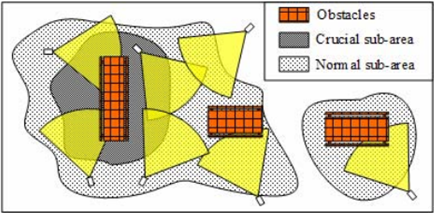
\includegraphics[width=\linewidth]{img/MapRoI165.png}
  \caption{ Map of an area to cover with  crucial sub area (region of interest) the normal sub-area  and obstacle. This map is an example of area coverage  introduce in  Jiang et al \cite{165*jiang2010}. 
.}\label{fig:MapRoI165}
  \endminipage\hfill
\end{figure}

The common point in all this coverage definition is the importance to maximize it, despite the other objectives. In the examples presented the coverage was always the first and for some of them the only objective. Despite the interest for maximize the coverage some other element have to be taken in account to have a useful cameras position depending on the finality. The secondary objective can have a not negligible impact on the camera pose. Depending on the camera pose will be greatly affected. The secondary objective are numerous and are closely related then the finality. The most interesting of them are listed:\\
\begin{itemize}
\item  The numbers of cameras: \\ In numerous situation the secondary objective is to limit the number of camera affected to the area as \cite{151*zhao2013,171*horster2006,22*zhao2008}. Limit the number of cameras is primordial to reduce the time computation for the final application and in some case the network traffic. Also reduce the number of camera to cover the full area mean reduce the cost of the video surveillance installation as \cite{82*chrysostomou2012}. In the case  minimizing the number of camera is a secondary objective not in contradiction with the camera pose optimization for coverage. The two objective can became complementary. But at some point a to strong trade-off in favour of the minimizing the numbers of cameras may reduce the area cover by accepting some small area  to be non covered (also called black hole). \\

\item Object tracking: \\ The secondary objective can be after the area coverage to detect and localize targets as for example in \cite{18*ding2012,12*soto2009,23*liu2009,39*wu2011,40*sohrabi2000,22*zhao2008}. In this case the secondary objective is to find a camera pose or dynamic adaptation of the pose for follow one or numerous targets. Keeping a full area covered and at same time the secondary objective is to track efficiently one or more target can became contradictory. The solution must be a trade-off between the coverage maximum coverage and the tracked following like in \cite{18*ding2012} and \cite{38*liu2010}. In Liu et al \cite{38*liu2010} the tracking of a target in a wide area is decomposed in phases, detection and location phase. For the detection phase, the area coverage is important but not any more for the location phase. These phases, although distinct for one target can intervene at the same time if there is more than one. Obviously when the secondary objective is to do tracking the cameras position will be less efficient for cover the area depending on the numbers of targets.  \\

\item  Luminosity and environmental setup:\\ Also  the  control of the image quality in terms of visibility can be an objective. Reddy et al \cite{33*reddy2012} are focus first on coverage of a complex area and in second time localize targets.  In order to manage what target must be follow the visibility is taking into account to avoid the too dark area, where the target is not enough visible at all. \\

\item  Energetic cost:
\\ To estimate the camera positioning another secondary element can be the energies cost in \cite{38*liu2010,42*bulusu2001}. Lui et al \cite{38*liu2010} is a good example, the first objective is to cover most of the area to be able to detect if a target is enter in the area. In second time the target is follow by the smart and autonomous cameras of the network. The set of cameras were randomly dispersed in the area and the coverage of the area will be to select the cameras useful for detect the targets intrusion in the area. The selection of the camera will be to manage between the maximum area overage and the minimum cost consumption.  Also the energy cost can be considered not in term of number of cameras turn on, but also in term of distance between each cameras. Notably in the case of each camera position will be a waypoint for doing a path planning \cite{191*di2016,218*meiting2007}.  
\\
\item Multi coverage:\\ Among the numerous secondary objectives possible the multi coverage is interesting (as for example in \cite{149*mavrinac2013,151*zhao2013,152*wang2009,174*zhang2016,175*medhi2013}). The multi coverage or also called K-coverage where $k$ represent the number of cameras useful to cover some region of the area. The multi coverage or $k$ coverage can be at some point confused with the region of interest and coverage priority. Mostly due to their importance given at some restricted part of area. The difference between them is the impact of the multi coverage on the finale coverage. The multi coverage involved one or few specific zone of the area to be covered by min $k$ cameras at same time in order to be considered as cover. This secondary objective in the case of limit will generate a conflict between the full coverage of the area and the k-coverage requirement even more with a restricted number of cameras. 
\\ 
\item  Resolution:\\ The objective of resolution is to keep the quality of the image acceptable \cite{27*bodor2005,33*reddy2012,171*horster2006,152*wang2009,43*erdem2006}. Most of his article are used the distance along the optical axis as a parameters in order to evaluate the resolution constraint. The lens, the sensor and the distance  between the camera  and a target (or surface) is used to estimate the resolution. In many application is essayer to adapt the distance between the camera and the target or the zoom (when the lens is not a fix focal ) then to modifies the other the sensor or the lens.\\
%The resolution is also model as the acceptable the depth of field.
  This secondary constraint affect mostly the system with positioning a set of cameras  comprising a zooming lens. If the constraint of resolution is not placed the interest to optimize the camera position for maximum coverage will be to zoom out (or place the camera highest) in order to cover  the wider region as possible. When the constraint of resolution is added a trade-off must be done between the zoom out or the camera distance to the target four maximize the coverage, and the zoom in to reduce the area cover for a better resolution.\\
   In \cite{33*reddy2012} the resolution is assimilated to be part of the image quality. In order to keep enough quality on the followed target,  the distance of the target is used to keep an acceptable resolution. The problem has been designed by using a Gaussian function in order to define the proper distance between the cameras and the target to keep an acceptable resolution for the application. \\
Also the depth of view have the same consequence on the camera positioning. Due to the focus point and the aperture of the camera (associate to the resolution), an object to close or to far became blurred. an ideal distance to the between the target and the camera is defined with some boundary  as in \cite{193*fu2014}. % (find ref 193)


\end{itemize}
The secondary objectives can be numerous and varied, where just few of them has been introduce (the more common and interesting). Among it, some of them are closely related and can be interconnected. The secondary objectives can be associate as in \cite{33*reddy2012} for example where the coverage target, luminosity, the resolution, and obstacle constraint are associate to find the best cameras position with maximize the coverage of the area and the target with good visibility condition. \\
The real interesting element about the secondary objectives is the impact in the cameras positioning for the global coverage of the area. Then the finality and the problem formulation will have a considerable impact of the obtained solution. Obviously the secondary objective have to be chosen carefully and there are related then the finality. To have an efficient cameras positioning system a trade-off between the different objective  and their importance have to be done in order to know what is the priority. In this case the problem became a multi objective problems. 


\section{Art gallery problem} \label{sec:AGP}
%Once the objectives defined the next step, is to know how to represent the problems. To do that manly 2 different class  of problems have to be studied. The first is from the geometrical problem called  the Art galery problms.

The problem of camera positioning is a tricky problem and depending on the finality of the camera networks and the formulation the camera pose will be affected.\\
 Once the objectives defined ( see section \ref{sec:camerasPositioning}) the next step, is to know how to represent the problems. To do that manly 2 different paradigms have to be studied.
 The first is from the geometrical problem called the Art Gallery Problem (AGP) formulation is commonly and historically borrowed as is presents in the following section with a fast definition of the problems, the solution used and the limit of this paradigm.


	\subsection{Definition of the paradigm}
	The art gallery problem is a geometrical problem introduced by Victor Klee in 1973. The problem was to estimate the number (and the position) of useful guard to cover an art gallery. 
The particularity of a art gallery is the complexity of the room shape, with many wall to dispose the painting. The shape complexity of the room make the estimation  of guards number even more difficult.\\
In order to formulate properly the problem, the room is assimilate at a polygon $P$, composed by $n$ vertices ($v_1; v_2;…v_n$). The vertices are linked by  $n$ edges ($v_1 v_2;…; v_{n-1} v_n$) to make  the shape of the Polygon $P$ (or room).

A guard $x$ is inside the room $x \in P$. A guard $x$ can cover or see any point $y \in P$ if the segment $xy$ is not intersect by any boundary of the polygon $P$ (wall), in order to have $ xy \subseteq P$.
The polygon $P$ is considered as fully cover when for any position of the point $y$ in the polygon at least one guard can see him.\\
A guard $x$ can cover at $360^\circ$ all around him, with no depth of field limitation (except the wall obstacle). Clearly that mean the guard can see and monitor the entire length of the room one side to another side if no obstacle around to occlude. For example, if the shape of the room is a triangle, quadrilateral or another convex simple polygon, at any position taken by one guard, this guard can monitor all the area despite the size of the room. 

The minimum number of guards $X$ useful to fully cover the polygons $P$ is $G(P)$ with $k$ is the number of guard in order to have a set of points $X=\{x_1…x_i…. x_k\}$ so that every $y\in P$  are cover by at least on point of the subset of $X$. \\
The AGP  in addition  to estimating the numbers of guard also are interested on finding the optimal position of this  restricted number of guard. 
This 2 questions can be solve in the same time by using one of the solution proposed.


	\subsection{Solution }
	
	The main advances on the AGP since this formulation in 1973 are numerous. The following paragraphs present the major advance on it.\\
	 The first and one of the more important is the proof given by Chvàtal in 1975 \cite{44*chvatal1975}.  The polygon must have to be covered by a minimum of guard, the proof of Chvàtal propose to link the minimum number of guards to the number of vertices $n$. 
A polygon composed by $n$ vertices need in the worst case a minimum number of guard equal at $n/3$ The Chvàtal proof is based on the triangulation of the polygon. The Triangulation is made based on the vertices of the polygon.\\
	 % For a polygon composed by $n$ vertices in the worst case the minimum guard necessary to cover it, is $X=n/3$.
	     The proof given by Chvàtal is also confirmed by the work of Fisk  few years later (1978). The work of Fisk is also based on triangulation and colouring node. It is probably the easiest to understand and also give a solution to estimate the pose of each guard ( it is recommended to begin by the Fisk proof before the Chvàtal despite the chronologic order as it is preconized in \cite{219*orourke1987}). The book of O'ROURKE et al \cite{219*orourke1987} is an early work about the AGP with the formulation, proof and advancement of the field clearly explained. \\
Once the proof of the minimum number in the worst case found the objective became to find an optimal solution in reasonable time. \\
For that the work of Toussaint and Avis (in 1981) is the reference and propose a solution working in $O(n log n)$. This work has been follow and upgrade until the solution of Couto, Resend and Souza  2011 \cite{224*couto2011} a solution is finally proposed in $O(n^3)$  in the worst case. 

It is a short overview of the AGP solution but also the solution proposed are very specific to the AGP and cannot be re-use for problem little different.

	
	\subsection{limit of AGP and camera coverage relation}


The problem of positioning camera for coverage estimation is quite close then the AGP. In many ways, the AGP is a reduction of the camera positioning for a total coverage of a complex areas. The camera positioning is the logical continuation of AGP and once some AGP is knew, the problem can be extended as is for  example show in \cite{221*fleishman2000,33*reddy2012,43*erdem2006}.

The algorithm developed for AGP cannot be applied directly on the problem of cameras positioning for maximum coverage. The main reason is the cameras limitation field and depth of view (\cite{82*chrysostomou2012,170*yabuta2008} which makes is unreadable the solution proposed of solve AGP, where AGP considering the guard with no limitation for the depth of field and field of view. \\
Also another reason make the AGP solution not applicable for the camera positioning is the diversity of cameras. In the same system the AGP may have many guard, they are all interchangeable because it has all the same ability (or skill) to monitor the area. This weakness in the AGP formulation associate to the limited field of view  make the solution form AGP note adapted as  is showed in \cite{81*nikolaidis2009,171*horster2006}.\\
Due to this limitation, the solution developed for AGP are not applicable. However the formulation and some proof has their importance. 
Despite that, numerous article are based on the AGP to formulate the problem as in \cite{43*erdem2006,53*packer2008}. For example in \cite{43*erdem2006} the similar approaches then the AGP is used  in order to estimate the occluded   region. Also in \cite{53*packer2008} (page 105)to estimate the area covered a grid of $y= (y_1 ...y_i)$ is used in order to discretise the area. this method is directly based on the AGP formulation.\\
Also one important impact of AGP is the shape of the room. In \cite{170*yabuta2008,171*horster2006,33*reddy2012,43*erdem2006} the shape of the room are close then the definition of an art gallery. This phenomena can be imputed to the link did between the number of vertices and the useful number of guards (or cameras) to cover it. \\
The room composed with numerous wall inside create few occlusion. The occlusion mean the segment $xy \not\subset P$   where $x \in P$ is the camera position $y \in P$ is a points in the room $P$. The occlusion is one of the element make the camera positioning really complex. The use of room inspired by  AGP is therefore a good choice in order to verify the effectiveness of the system in a complex environment.\\
The complexity of this problem is also an important factor which makes the relation of camera positioning and AGP. \\
The AGP is NP-hard problems \cite{219*orourke1987}). The NP-hard proof is available on the book of O’Rourke section 9.2 of the book \cite{219*orourke1987}). \\
To proof the AGP is  NP-hard, the first part is to reduce the  problem to an other problem welle known for this complexity. The relation is made by reducing the AGP with a polygon composed by  holes to another standard problem ( in the demonstration the is used 3SAT). \\
Once the AGP is reduced to 3SAT and because 3SAT is an NP-complete problem the AGP is  also considered as NP-complete or  NP-hard but only  when the room is composed with holes. Also another work of Lee and Lin 1986 proof the complexity of AGP without hole also by reducing the AGP ton an other well known problem (for more explication see the book of O’Rourke  section 9.3 \cite{219*orourke1987})).

As we explained earlier the camera positioning can be reduced as an AGP \cite{53*packer2008} notably by removing most of the constraint due to the camera properties. \\
In the literature numerous article us the AGP reference to explain the complexity of the problem as for example \cite{26*moeini,44*chvatal1975,149*mavrinac2013,151*zhao2013}  assumed the problem is at least NP-complete or NP-hard. 
The complexity of the problem will have an impact on the solution used  to try to solve it and optimize it.

The AGP can be at same time  for part the  historical source of the cameras positioning and give some answer about the problem this formulation and this complexity. Despite that, the AGP is not the only source to refer about the cameras positioning for maximize the coverage. Some clue and solution can be find in other related field. 




\section{Wireless sensor network   }

The wireless sensor network (WSN) can be as AGP considered as inspiration for the cameras positioning problem. The WSN is an active field of research and in many aspect related to the cameras positioning. This parties is focused on the WSN and this relation with the camera positioning.  But first allow  :

What is the Wireless Sensor Network? 

 The WSN is a distributed network of sensor or in some case actuator, in this case is also called WSAN. Each sensor of the network is a relay for the information and commend, to the rest of the network.  
The sensor are at same time the node for the network. The node have to objective to transmit by relaying the information to the other node or to a centralized agent.  Furthermore the node have to be the sensor for collect information and decided to communique with the other node. 
The information collected by the sensor are vast (extensive) depending on the final application and the capacities of the sensors ability. 
The WSN is used in different field for various application as for telecom and antenna positioning \cite{59*wang2008} military surveillance field \cite{38*liu2010,101*topcuoglu2009}, airport surveillance \cite{37*ma2012}, video surveillance and tracking \cite{38*liu2010}, environmental monitoring \cite{42*bulusu2001}... Logically numerous sensor and information can be collected  as temperature, movements, images, song and also some  actuator can be used as radio frequency for example.\\
 The application of WSN are wide, especially since the WSN has more than one discipline. The WSN try to optimize a network of sensor in different aspect as for example \cite{39*wu2011} focus on an architecture adapted and efficient enough for data transfer (image) or like in \cite{40*sohrabi2000} the WSN are dedicate to adapt the network around static node and energetic resources in order to keep the network connected.  \\
For our case the discipline the more interesting is the coverage of an area with his specific constraint of the WSN for maximum coverage.\\
 The other discipline of the WSN as the network optimisation will not be addressed in the following section. Only the problem of coverage is studied  the other discipline are not considered as the first or main objective but can be some secondary objectives after the problem of coverage.

	\subsection{Sensor at 360}
	\begin{figure}[t!]
\minipage{0.55\textwidth}
   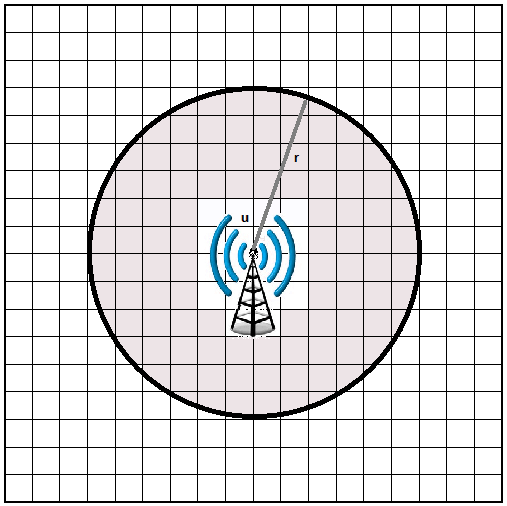
\includegraphics[width=\linewidth]{img/WsnSensor1.png}
  \caption{ one omnidirectional sensor centred on $u$, with a radius $r$ for the range.}\label{fig:WsnSensor1}
  \endminipage\hfill
\end{figure}

The wireless sensor network (WSN) refer commonly to sensor or actuator  with no restriction in the view angle, it is considering to have a $360^\circ$ of field of view  as in \cite{200*kulkarni2011, 174*zhang2016,150*chakrabarty2002} (see Figure \ref{fig:WsnSensor1}) and in some case a spherical as example in \cite{175*medhi2013,59*wang2008}.  \\

Each sensors have a position $u$ in the area and a power. From the sensor power the radius $r$ of the circle is deduced from $u$ as center (show \ref{fig:WsnSensor1}). This circle give the area cover by a sensor in the simplest case. 
The simplest case correspond to a flat area without any obstacle, or it is negligible and do not impact the covered area as in \cite{200*kulkarni2011,174*zhang2016}.  
Others more complex solutions can be used. Its are more complex but also more realistic as in \cite{59*wang2008} where are taking in account the relief and obstacle. 
In \cite{174*zhang2016} more complex model have been developed, where despite of a flat ground without obstacle each sensor is composed by a perception radius and a communication. The communication radius a bit bigger then the perception radius. This 2 radius correspond to area covered for one antenna (sensor) and the distance of emission/reception of the data.  In order to have an efficient coverage of the area, the antenna must be place in order to have connection with other antenna but without too much overlap of the perception sensor.\\

The solution proposed in order to optimize the positioning of the WSN for a circular sensor can be varied. Mostly 2 different ways are applied for the sensor with have circular angle of view or spherical.\\

\begin{itemize}



\item	The first solution use an heuristic based on geometry construction as in \cite{175*medhi2013}. This approaches give a good coverage solution but is usually greedy and can be quickly limited in term of number of sensors, moreover if some external constraint are added.  For example in \cite{174*zhang2016} the greedy solution was tested and optimized by using a "partition and shifting" strategy in order to upgrade the result.
The limit of this solution despite the greedy consumption resources is also not applicable to the problem of camera positioning due to the reduced field of views of a cameras.  \\
\item	The second solution try to find an efficient and quick solution to optimize  random position for each sensor of the network.  
This solution include many different family of algorithms focused on optimization.
Among the family of algorithms,  the evolutionary algorithms (disused in detailed in section  \ref{chap:EA}) is commonly used as in \cite{200*kulkarni2011,59*wang2008}, and \cite{150*chakrabarty2002}. \\
These solutions  propose to optimize the position in order to maximize the coverage depending on different constraint or the secondary objectives. The method of optimization have to be adapted to the problem. 
In  \cite{150*chakrabarty2002} the integer linear programming with an "LPsovlver" are chosen in order to maximize the coverage with 2 type of sensors. One standard with a smaller area coverage but with a smaller cost (can have a $100m$ radius for 150\$) and the other sensor can cover a wider region (can have a $200m$  radius for 200\$) and the objective is to cover the region but also to reduce the cost. The solution proposed is to use the integer linear programming adapted to the problem of coverage optimization with the economic cost in constraint. \\
In \cite{59*wang2008} and \cite{200*kulkarni2011} the solution proposed is based on 2 different evolutionary algorithm in order to optimize the sensor positioning. In \cite{200*kulkarni2011} the camera positing with a multi coverage is solved with using an evolutionary algorithm called particle swarm optimization (PSO). The objective is to optimize the position of the sensor in order to have an efficient coverage of the area and also enough redundancy to keep the network workable if one or few sensor fail. In \cite{59*wang2008} one evolutionary algorithms is also used to optimize the potion of antenna. The objective in this paper is to give the best coverage of an area with taking in count the relief of the area. The relief make the coverage estimation of each sensor even more complex and costly in terms of time computation. The Genetic algorithm are used in order to find quickly a position for each antenna of the network. 
\\
\end{itemize}

Among the examples seen the second solution based on optimization is the more interesting and also the more flexible to new constraints and secondary objective. The aim is to see up to what point and if it is applicable to the problem of cameras network positioning.  

	\subsection{Visual sensor network}
	
Logically, the result obtained with the Omni-directional sensor are interesting and  must be applied to the problem with even more constraint and objective as can be the  positioning of visual sensor network (VSN).  In fact the visual sensor or camera have a limited depth of field but also a limited field of view. This new constraint make the sensor positioning more complex as that was for AGP (see section \ref{sec:AGP}) to passes from guard to camera. The advantage in this case,  are first the sensor have been designed with a limited depth of field. Also the solution applied previously for circular sensor was not only geometric or based on heuristic but also the problem is formalized as optimization problems with some solution based on optimization and meta-heuristic. This way to present the problem is appear as the more suitable to add constraint and secondary objectives. Also the solution and the formulation for the problem of VSN are mostly the same then the problems of cameras positioning and is  discussed in the following parts  \\
  

	\section{Solution not based on evolutionary method}
	
The solution used to pose a set of cameras to maximize the coverage are various but  among the possible solution manly two way can be describe. The solution proposed they come from numerous sources and paradigm  which AGP and WSN.\\
 The first is to construct a solution as an heuristic to have an appropriated cameras position. The second way is to formalize the problem as optimization problem and applied meta-heuristic. 

\subsection{The constructive solution}

The cameras pose can be done by construction. By construction that mean a deterministic method is applied to pose one camera after the other or to adjust their position.\\
In \cite{38*liu2010} a constructive solution is applied in order to select the smart cameras of the network. Each smart camera area a node of the network and transmit information, image and are fully autonomous. 
They work in 3 different modes:\\
\begin{itemize}
\item[-] The first is the sleepy mode. The sleepy mode is used in order to economize a maximum of the energy. To do that the camera is turn off. That mean no computation and just the network is listen at regular intervals to wait the wakeup call.   \\

\item[-] The Second is the detection mode the camera is turn on, but with a low frame rate. Just a few computation is done to detect if a target is enter in the field of views. Some information may be transmit by network. This mode consume more energy of the previews but the smart cameras can stay in this mode during a long time.\\

\item[-] The last mode is a tracking mode. This mode is the more energy consumer. The camera is turn on, with a high frame rate and numerous computation have been done to track and localize the target. Also more information have to be transmit by the network. The information are useful to localize the target by communicate with  the potential other smart cameras with a view on the target. \\
\end{itemize}
The objective in \cite{38*liu2010} are multiples depending on the state of the cameras. the one the more interesting for us is to keep under control the longest time as possible the area for target detection. Numerous smart camera are randomly dispersed in the area (as an air-drop in a battlefield) and the aim is to select the camera in order to maximize the coverage of the camera in detection mode. The solution proposed by LIU  et al in \cite{38*liu2010}.
To do that the solution used is by construction with using a talk between each smart cameras of the network. Also each sensor is capable to estimate precisely this localization, it is an important element to select the cameras. The solution proposed is inspired of the network distributed talk. \\
To begin all sensor are in sleepy mode.  The camera wake up regularly and send a call at the neighbour, if they receive no answer that mean no other camera is awake around and the camera stay in detection mode. If no enough answer have been received, that mean the required density of the camera around are not enough the camera stay turn on detection mode. Otherwise the camera return on sleepy mode until another wake-up later. This procedure is applied in each smart camera with all have their own pace. After a certain time the network is well organize to cover the area in detection mode.
 The method introduce by LIU et al in \cite{38*liu2010} work well. the solution proposed have the advantage to can  work in wide area and to be dynamic (if one cameras do not have any-more power the network ll re-adapts).  \\
The solution are efficient  with a high density of sensor to have a relatively low coverage (just enough to detect target in the sparse sensor placement). Also the method presented is really dependent then the network communication and the capability to localize precisely each sensor. Finally the solution proposed to select a set of sensor among a randomly posed sensor is not enough optimized.\\

Another cameras pose estimation by construction is proposed by HÖRSTER et al \cite{171*horster2006}.
The solutions proposed is based on a greedy search heuristic.  The objective is to find a position and orientation of a set of cameras with a fixe pan, in the environment inspired by the AGP. \\
In \cite{171*horster2006} a first greedy search solution have been presented then finally a solution called Dual Sampling has been presented based on it.
The dual sampling is an incremental method. \\
First step is to initialize the position of all the cameras. A random initialization for the position and the orientation must be appropriate.  \\
Second step is to select one point of the area. The area is discretized by numerous points, with each point must be covered by at least one camera. Around the selected point several position and orientation are tested for the cameras at proximity. The possible position are obtained by sampling the area around the point to cover. Finally the best cameras position and orientation is kept.
The second step is repeated and the set of uncovered control point is reduced an each iteration.  This procedure is applied until the stop criterion is reach that mean enough points of the area are covered. \\
This constructive solution have some inconvenient notably in terms of efficiency. Indeed this solution is limited by the number of camera and size of the area due to the exponential complexity.\\

In \cite{81*nikolaidis2009} the camera placement to cover a basic mobile robot trajectory is studied.
The trajectory is modelled as the region of interest, with a gradually decreasing interested from the trajectory center.\\
  The solution applied in  \cite{81*nikolaidis2009} is to do a local optimization one camera after the other with the “steepest decent method (decent de gradient)”. If this local optimization give a better solution the network of camera is modified otherwise the camera stay at the same place. This operation is repeated until the convergent arrangement is obtained or no more upgrade can be found. This result presented in the experiment done by Nikolaidis in  \cite{81*nikolaidis2009} are interesting despite the simplicity of the area and the very small amount of camera used.  The principal limitation is due to the number of step required for optimize independently each camera of the network. Also a multitude of local optimisation is not obviously the same then the global optimization.\\

Ma et al \cite{37*ma2012} propose a solution for the problem of finding the minimum camera barrier coverage. The objective is to cover only the boundary of an area, to be able to detect target intrusion in the perimeters. The perimeter is relatively wide and can be considering at some point as an area to cover composed by big hole in this center.\\
 The region to cover is cut in numerous sub-region. The region are inter connected, each sub-region have to be “full-view covered”. The full view covered is define if for any target direction there always exist a sensor cover to the face of it.\\
The solution purposed is based on constructive solution with adapted heuristic (the heuristic used is presented on \cite{37*ma2012}). The global idea is to cut the perimeter in different sub-region and applies the method presented to full view cover  each sub region. 
The cutting on sub-region offer at the heuristic to work in reasonable time due to this restricted area.\\
The solution proposed though this efficiency in the case of barrier coverage is not rely appropriate to vast coverage area. The first limitation is the number of cameras use to fully cover the area. The number of cameras is mainly due to this definition of “full view covered” . That definition  imply many overlap to have the multi direction coverage.\\


As show, the previous solution are based on constructive method for the camera placement and their local optimization. Each camera is placed dependently then the network with an iterative process in order to have a position for each camera of the set. This methods have some consequence, nobly the fast increasing number of iteration useful to have a solution good enough. The time complexity is event more problematic with  increasing the size of the area. Also these solution are extremely dependent then the formulation and the constraints and cannot be easily adapted to other problems. 

\subsection{ !!! Linear programming optimisation !!! (to verify)}
	Different method of linear optimization was applied and test. In some case due to a well-adapted formulation; a specific shape of the area or cameras number The linear optimisation is efficient. 
	The linear optimisation has been commonly used to have initial result in order to have a reference point before to develop other solution more appropriate(as example \cite{141*akbarzadeh2013,151*zhao2013,82*chrysostomou2012,33*reddy2012}…).  \\
%	The reason ofIn some other case the method was studied but finally rejected du to this fast limitation 
	 The linear optimisation  is finally rejected due to this fast limitation.  Indeed the linear optimization can be quickly in difficulty due to the fast increasing complexity of the problem and in many case be lock in local minima. as presented in the flowing example.\\

%%\textbf{!!!!!! partie manguante sur l'utilation des methode linear  !!!!!(voir path planning)}
	 
	 
The \cite{43*erdem2006} is based on AGP and the WSN and propose a fusion off their 2 paradigms in order to use there assumptions. Some modification have been done as example to taking in account the field of view limitation. The interesting aspect is how some camera properties have been modeled to fit to the problem of AGP.  \\
The solution proposed is workable with using an omnidirectional or considering a PTZ as omnidirectional cameras by using an efficient angular sweep. The simulated omnidirectional cameras is simulate by PTZ camera with a non-continue zoom or fix focal length as in the  experimentation (see fig 7) where  the PTZ can have a focal two focal length  at 50mm and  35mm. 	 \\
	 

Finally the solution proposed is to discretize the area to cover (fig 7 left) and also the different possible parameter for the camera (as: localization, orientation, focal...). Thanks to this discretization and a formulation close then the binary integer programming (BIP) and apply a well-known method “Branch and Bound” in order to optimize the camera placement.  \\
This solution  propose a  good  coverage with the minimum of cameras  in reasonable time until, the  number of location sample ( point in the grid on the floor) , the numbers of camera, and the number of parameter possible for the camera stay relatively  reduced.  \\
 
Zhao  et al \cite{22*zhao2008} are trying to find the optimal position for a set of camera in order to maximize the  Indore coverage (like an AGP room) and also to  do tag detection.
The solution proposed for the coverage is to adapt the number of point of interest wish must be covered by the camera. \\
The area is discretize in grid.  The grid is composed by point selected smartly depending on the coverage rate. Each point of the grid simulate a potential location of the target.\\
Also a limited number of possible position for the camera (the boundary of the room) are defined.
The adapted grid and the limited camera positioning is used to limit the complexity ( as number of possible solution).  linear optimization to the Binary integer problem formulation. \\
Use a Binary integer problem formulation (BIP) in order to apply a linear optimization is popular and other use it as in \cite{22*zhao2008,27*bodor2005,43*erdem2006}. In \cite{22*zhao2008} the solution proposed is to use BIP formulation the grid smart sampling and LP\_solve to optimize the camera position and orientation.\\

 A Similar method is used in \cite{27*bodor2005} to find the position and orientation of a set of cameras. The goal of this paper is to find the appropriate position with maximize the resolution for a set of cameras dedicate to do tracking. The position is determined depending on a set of standard pedestrian trajectories. The camera pose try to maximize the given trajectory to have the best resolution and the entire coverage. \\
The problem is also formulate in order to apply a linear well-known algorithm. In this case the branch and bound is applied.  

\subsubsection{	Limitation of linear method}
Different method of linear optimization was applied and test to answer, the problem of camera position for maximum coverage. In some case due to a well-adapted formulation or a restricted area and cameras number this solution is efficient enough. In some other case the method was studied but finally rejected due to this fast limitation (as example \cite{141*akbarzadeh2013,151*zhao2013,82*chrysostomou2012} …). Indeed the linear optimization can be quickly in difficulty due to the fast increasing complexity of the problem and in many case be lock in local minima.

	
In WANG et al \cite{181*wang2017} propose a solution with an atypical problem formulation. The solution proposed in \cite{181*wang2017} is mainly based on the method of discretize the area. The idea is to have an area discretized with precision with use the minimum of point. To do that the solution proposed is to decompose the area in order to give more point in the grid were the shape of the room need it to be correctly described. \\
The principal advantage of this solution is to propose an area representation with enough precision and a minimum of point to describe it. Less point to describe the area to cover mean also a winning time efficiency in computation during the camera pose estimation (cost function is faster).
Despite this interesting solution the result presented in the experiment does not appear to be conclusive. \\
	
\subsection{Game theory} 
	 
Among possible solution an atypical method is to use the game theory \cite{19*li2013}. The game theory is use to optimize the looking direction of the cameras as in \cite{12*soto2009,18*ding2012,19*li2013,25*song2008}. These articles are based on game theory to find an equilibrium (also named Nash equilibrium) between two contradictory objectives, the maximize the resolution and the multi target tracking.\\

Soto et al \cite{12*soto2009} propose a network of a dozen of PTZ cameras. The PTZ is for pan tilt zoom, that mean the position of the cameras are fix and the solution proposed is to find the best orientation with the appropriate focal lens to track most of the targets.  \\
 To do that the camera are smart enough to communicate with the close neighbours and adapt the pan, tilt, zoom depending on the needs.\\
The need has been defined by an utility function (or local cost function). The goal is to track most of the target as possible with the better resolution. The cameras scores when it obtained a desired resolution image for all the targets visible by the networks.\\
The trade-off proposed is between the multi tracking and the best coverage resolution for each target. The multi-target problematic can appear far from maximization of the coverage. But the number of targets  which may be higher than the number of cameras, push the camera tracking to be an interesting solution to maximize the coverage of an area. In this case the quality of the coverage will also dependent then the number of targets and the importance of the resolution constraint.  \\
	 In \cite{18*ding2012} and \cite{25*song2008} different experiment have been proposed with a number of target is lightly increased.  In this articles the game theory is applied to trade-off between the tracking and the resolutions. The proposed experiment is based on the decentralized method. It is justified by the complexity to dynamically adapt all the camera of the network at same time depending on each targets trajectories.\\
	  Furthermore, the decentralized solution is more adapted for the security of the transmission and the risk of interception by a hostile opponent. The security may be an important factor in some applications. \\
To have the decentralized system the camera must have some autonomy. \\
In the experiment proposed in \cite{12*soto2009} and \cite{18*ding2012,25*song2008}  each camera are smart enough to have their own tracking  and control module. Also the camera are able to communicate with each other to come to a consensus. The consensus is when a Nash equilibrium is found between the 2 contradictory objectives. In this case it is a win win situation for both objectives.\\
So the objectives are not independently optimize, moreover  the  solution proposed is to optimize its  simultaneously in order to have a consensus. The consensus is reach when it became impossible to upgrade one of them without downgrade the other one.\\
  In the experiment of \cite{18*ding2012,25*song2008} the consensus is found by the camera communication in order to have a maximum of the target cover with the higher resolution.
 The experiment is based on numerous target moving freely in the area. Also in \cite{18*ding2012} one of the target must be cover in priority with a high resolution. That will have an impact on the other camera position.
 The result of the experiment as in figure \ref{fig:CoverageFrom18} form \cite{18*ding2012} show a really efficient global coverage with almost all the target cover at every time despite the movements of the targets. \\
 The advantage of these solutions is the acceptable result and dynamic reconfiguration of the system for the reasonable size of the area and the decentralized computation.\\
Otherwise this method have some limit, as show in the experiment the area is relatively restricted and numerous cameras with a fixed position are useful. The consequences is the quantity of overlap relatively important. In this case the number of sensor is not well optimize to cover the area. Also to use properly this method for maximum coverage it requires a large number of simulated target in the region to observe. 

\begin{figure}[t!]
\minipage{0.55\textwidth}
   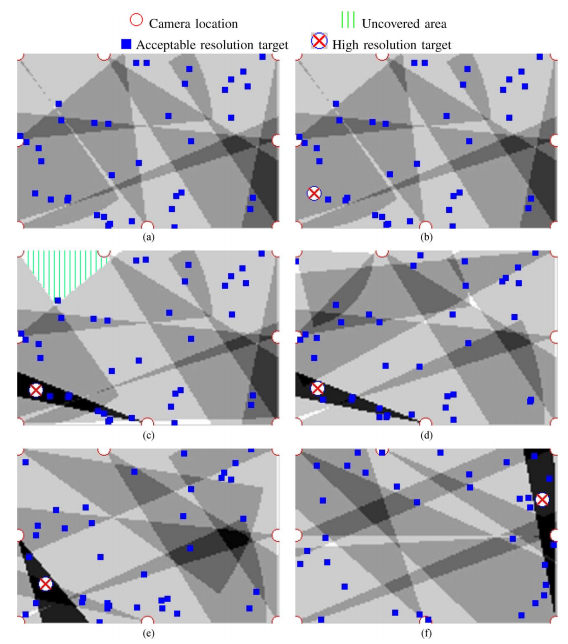
\includegraphics[width=\linewidth]{img/CoverageFrom18.png}
  \caption{ result of coverage after have used the game theory with objective to maximize the tracking and the resolution. result obtained in the experiment presented in \cite{18*ding2012}}\label{fig:CoverageFrom18}
  \endminipage\hfill
\end{figure}
	
	%%%%%%%%%%%table sum up%%%%%%%%%%%%%%%%%%%%%%%%%%
	% Please add the following required packages to your document preamble:
% \usepackage{booktabs}
% \usepackage[table,xcdraw]{xcolor}
% If you use beamer only pass "xcolor=table" option, i.e. \documentclass[xcolor=table]{beamer}
%\begin{landscape}
%
%	\begin{table}[]
%\centering
%\caption{Sum up articles.}
%\label{my-label}
%\begin{tabular}{@{}lp{2.6cm}lllp{1.6cm}p{1.6cm}llp{1.3cm}p{1.3cm}p{1.65cm}p{1.6cm}p{1.3cm}p{1.3cm}p{1.4cm}@{}}
%\toprule
%\multicolumn{1}{|l|}{\textbf{ref}}               & \multicolumn{1}{l|}{\textbf{\begin{tabular}[c]{@{}l@{}}Best \\ solution\end{tabular}}} & \multicolumn{1}{l|}{X} & \multicolumn{1}{l|}{Y} & \multicolumn{1}{l|}{Z} & \multicolumn{1}{l|}{\begin{tabular}[c]{@{}l@{}}Point\\  selection\end{tabular}} & \multicolumn{1}{l|}{Pan} & \multicolumn{1}{l|}{Tilt} & \multicolumn{1}{l|}{Roll} & \multicolumn{1}{l|}{focal lenght} & \multicolumn{1}{l|}{\begin{tabular}[c]{@{}l@{}}Coverage\\  representation\end{tabular}} & \multicolumn{1}{l|}{\begin{tabular}[c]{@{}l@{}}number of \\ cameras\end{tabular}} & \multicolumn{1}{l|}{\begin{tabular}[c]{@{}p{1.65cm}@{}}Secondary objectives \\ and contraints\end{tabular}} & \multicolumn{1}{l|}{} & \multicolumn{1}{l|}{} & \multicolumn{1}{l|}{} \\ \midrule
%\rowcolor[HTML]{FFFFFF} 
%\multicolumn{1}{l|}{\cellcolor[HTML]{FFFFFF}37*} & heurisitic                                                                             & x                      & x                      & 0                      & 0                                                                               & x                        & 0                         & 0                         & fix                               & 2D                                                                                      & around 10 (per section)                                                           & barrier coverage                                                                                    & conection dependance  &                       &                       \\
%\multicolumn{1}{l|}{\cellcolor[HTML]{F2F2F2}38*} & \cellcolor[HTML]{F2F2F2}heuristic                                                      & \cellcolor[HTML]{F2F2F2}0                      &\cellcolor[HTML]{F2F2F2} 0                      &\cellcolor[HTML]{F2F2F2} 0                      & \cellcolor[HTML]{F2F2F2}\begin{tabular}[c]{@{}l@{}}random \\ dispersion (x;y)\end{tabular}              &\cellcolor[HTML]{F2F2F2} 0                        &\cellcolor[HTML]{F2F2F2} 0                         &\cellcolor[HTML]{F2F2F2} 0                         &\cellcolor[HTML]{F2F2F2} fix                               &\cellcolor[HTML]{F2F2F2} 2D                                                                                      &\cellcolor[HTML]{F2F2F2} around 600                                                                        & \cellcolor[HTML]{F2F2F2}resolution                                                                                          & \cellcolor[HTML]{F2F2F2}tracking              &  \cellcolor[HTML]{F2F2F2}                     &                      \cellcolor[HTML]{F2F2F2} \\
%\rowcolor[HTML]{FFFFFF} 
%\multicolumn{1}{l|}{\cellcolor[HTML]{FFFFFF}27*} & non-linear                                                                             & x                      & x                      & 0                      & 0                                                                               & x                        & 0                         & 0                         & fix                               & 2D                                                                                      &                                                                                   & tracking                                                                                            & resolution            &                       &                       \\ \rowcolor[HTML]{F2F2F2}
%\multicolumn{1}{l|}{ \cellcolor[HTML]{F2F2F2}43*} & \cellcolor[HTML]{F2F2F2}game                                                           & x                      & x                      & 0                      & 0                                                                               & x                        & 0                         & 0                         & x (discret)                       & omni directional (mobil pan)                                                             & around 10                                                                         & cost reduction                                                                                      & resolution            & DoF                   &                       \\
%12*                                              & game theori                                                                            & 0                      & 0                      & 0                      & 0                                                                               & x                        & x                         & 0                         & x                                 & 2D                                                                                      & around 10                                                                         & resolution                                                                                          & tracking              & multi target          &                       \\
%\rowcolor[HTML]{F2F2F2} 
% 18*                                              & game theori                                                                            & 0                      & 0                      & 0                      & 0                                                                               & x                        & x                         & 0                         & x                                 & 2D                                                                                      & around 10                                                                         & resolution                                                                                          & tracking              & multi target          &                       \\
%25*                                              & game theori                                                                            & 0                      & 0                      & 0                      & 0                                                                               & x                        & 0                         & 0                         & x                                 & 2D                                                                                      & around 14                                                                         & resolution                                                                                          & tracking              & multi target          &                       \\
%\rowcolor[HTML]{F2F2F2} 
%81*                                              & heurisitic                                                                             & x                      & x                      & 0                      & 0                                                                               & x                        & 0                         & 0                         & fix                               & 2D                                                                                      & 2 to 4                                                                            & Region of interst                                                                                   & trajectory coverage   &                       &                       \\
%22*                                              & LP-solve                                                                               & x                      & x                      & 0                      & 0                                                                               & x (16 orientation)       & 0                         & 0                         & fix                               & 2D                                                                                      & around 10 (8-11)                                                                  & tag detection                                                                                       & tag visbility         &                       &                       \\
%\rowcolor[HTML]{F2F2F2} 
%170*                                             & linear programming relaxation                                                          & x                      & x                      & 0                      & 0                                                                               & x                        & 0                         & 0                         & fix                               & 2D discret square                                                                       & around 20                                                                         & Region of interst                                                                                   &                       &                       &                       \\
%171*                                             & LP-solve                                                                               & x                      & x                      & 0                      & 0                                                                               & x                        & 0                         & 0                         & x (discret 3)                     & 2D                                                                                      & around 10                                                                         & cost reduction                                                                                      &                       &                       &                       \\
%\rowcolor[HTML]{F2F2F2} 
%181*                                             & Multistage Grid Subdivision                                                            & x                      & x                      & 0                      & 0                                                                               & x                        & x                         & 0                         & x                                 & 2D                                                                                      & 9 to 15                                                                           & Region of interst                                                                                   & big area              &                       &                       \\ \cmidrule(r){1-13} \cmidrule(l){16-16} 
%\end{tabular}
%\end{table}
%	
%\end{landscape}	
	
	
	%%%%%%%%%tab v2 %%%%%%%%%%%%%%%%%%%%%%%%%%%%%%
\begin{landscape}	
	\begin{table}[]
\centering
\caption{Sum-up ref}
\label{tab:sum-up1}
 %              ref           |x|y |z| pan|      tilt| |focal  coverage     nmb   
\begin{tabular}{@{}l|p{2.4cm}  l  l l p{0.659cm}p{0.62cm}lp{1.3cm}p{1.57cm}p{1.5cm}p{1.6cm}p{1.3cm}p{1.2cm}@{}}
\toprule
\multicolumn{1}{|l|}{\textbf{ref}} & \multicolumn{1}{l|}{\textbf{\begin{tabular}[c]{@{}l@{}}Best \\ solution\end{tabular}}} & \multicolumn{1}{l|}{X}              & \multicolumn{1}{l|}{Y}              & \multicolumn{1}{l|}{Z}             & \multicolumn{1}{l|}{Pan} & \multicolumn{1}{l|}{Tilt} & \multicolumn{1}{l|}{Roll} & \multicolumn{1}{p{1.29cm}|}{focal lenght} & \multicolumn{1}{l|}{\begin{tabular}[c]{@{}p{1.55cm}@{}}Coverage\\  room\end{tabular}} & \multicolumn{1}{l|}{\begin{tabular}[c]{@{}l@{}}number\\ of \\ cameras\end{tabular}} & \begin{tabular}[c]{@{}l@{}}Secondary objectives \\ and constraints\end{tabular} &                      &               \multicolumn{1}{l|}{} \\ \midrule
\rowcolor[HTML]{FFFFFF} 
\cite{37*ma2012}                        & heuristic                                                                             & x                                   & x                                   & 0                                  & x                        & 0                         & 0                         & fix                               & 2D                                                                                      & $\approx 10                                                                        $                                                           & barrier coverage                                                               & conection dependance &                                     \\
\rowcolor[HTML]{EFEFEF} 
\cite{38*liu2010}                                & heuristic                                                                              & \multicolumn{3}{l}{\cellcolor[HTML]{EFEFEF}\begin{tabular}[c]{@{}l@{}}random \\ dispersion (x;y)\end{tabular}} & 0                        & 0                         & 0                         & fix                               & 2D                                                                                      & $\approx 600                                                                        $ & resolution                                                                     & tracking             &                                     \\
\rowcolor[HTML]{FFFFFF} 
\cite{27*bodor2005}                                & non-linear                                                                             & x                    & x                                   & 0                                  & x                        & 0                         & 0                         & fix                               & 2D                                                                                      &                                                                                   & tracking                                                                       & resolution           &                                     \\
\rowcolor[HTML]{EFEFEF} 
\cite{43*erdem2006}                               & game                                                                                   & x                                   & x                                   & 0                                  & x                        & 0                         & 0                         & x \newline(discret)                       & omni directional (by pan)                                                             & $\approx 10                                                                        $ & cost reduction                                                                 & resolution           & DoF                                 \\
\rowcolor[HTML]{FFFFFF} 
\cite{12*soto2009}                              & game theory                                                                            & 0                                   & 0                                   & 0                                  & x                        & x                         & 0                         & x                                 & 2D                                                                                      & $\approx 10                                                                        $ & resolution                                                                     & tracking             & multi target                        \\
\rowcolor[HTML]{EFEFEF} 
\cite{18*ding2012}                                & game theory                                                                            & 0                                   & 0                                   & 0                                  & x                        & x                         & 0                         & x                                 & 2D                                                                                      & $\approx 10                                                                        $ & resolution                                                                     & tracking             & multi target                        \\
\rowcolor[HTML]{FFFFFF} 
\cite{25*song2008}                                & game theory                                                                            & 0                                   & 0                                   & 0                                  & x                        & 0                         & 0                         & x                                 & 2D                                                                                      & $\approx 14                                                                        $ & resolution                                                                     & tracking             & multi target                      \\
\rowcolor[HTML]{EFEFEF} 
 \cite{81*nikolaidis2009}                      & heurisitic                                                                             & x                                   & x                                   & 0                                  & x                        & 0                         & 0                         & fix                               & 2D                                                                                      & 2 to 4                                                                            & Region of interst                                                              & trajectory \newline coverage  &                                  \\
\rowcolor[HTML]{FFFFFF} 
\cite{22*zhao2008}                    & LP-solve                                                                               & x                                   & x                                   & 0                                  & x        & 0                         & 0                         & fix                               & 2D                                                                                      & $\approx 10                                                                        $ (8-11)                                                                  & tag \newline detection                                                                  & tag \newline visbility        &                                  \\
\rowcolor[HTML]{EFEFEF} 
\cite{170*yabuta2008}                              & linear\newline programming \newline relaxation                                                          & x                                   & x                                   & 0                                  & x                        & 0                         & 0                         & fix                               & 2D\newline discrete square                                                                       & $\approx 20                                                                        $                                                                          & Region of interst                                                              &                      &                                     \\
\rowcolor[HTML]{FFFFFF} 
\cite{171*horster2006}                               & LP-solve                                                                               & x                                   & x                                   & 0                                  & x                        & 0                         & 0                         & x \newline(discret)                     & 2D                                                                                      & $\approx 10                                                                        $ & cost reduction                                                                 &                      &                                     \\
\rowcolor[HTML]{EFEFEF} 
\cite{181*wang2017}                               & Multistage Grid Subdivision                                                            & x                                   & x                                   & 0                                  & x                        & x                         & 0                         & x                                 & 2D                                                                                      & 9 to 15                                                                           & Region of interst                                                              & big area             &                                     \\ \bottomrule
\end{tabular}
\end{table}
\end{landscape}	
	%%%%%%%%%%%%%%%%%%%%%%%%%%%%%%%%%%%%%%%%%%%%%%%%%%
	
	
	\section{Solution based on evolutionary  method.} \label{sec:SolutionBasedonEA}
	
	The solution already broach formulate the problem of camera positioning (as in the section 2.4) from various point of views. But the more common have not been approach yet.
In numerous work the camera positioning for maximum coverage is assimilated to a problem of optimization. Due to the complexity of the problem (as that was introduce in the AGP section \ref{sec:AGP}) the linear optimization may not appropriate.  
The solution is to apply some stochastic method with an appropriate meta-heuristic. Among the various possibility the algorithm from the Evolutionary algorithm has been used at numerous time. 

In \cite{151*zhao2013} different solution have been tested to optimize the position. Among the solution proposed a greedy with a local optimization,  a sampling algorithms and the Simulated Annealing (SA) from the EA family has been compare.  Also the SA is used to customize the sampling mechanize in order to propose a new customized solution. \\
In Zhao et al \cite{151*zhao2013}, the problem is formalized as a BIP (binary integer programing). %The  optimization methods have been applied to find the best position and orientation for the set of cameras.
  The goal is to find among a restricted numbers of possible positions and orientations the best pose for a set of cameras. To cover the area, despite the obstacle and the region of interest. \\
Among the solution proposed, the greedy algorithm has a good approximation until the number of camera stay relatively small. The problem of the greedy algorithm is to have an important risk to be stock in the local optimum. This risk increase proportionally then the size of the environment. Otherwise the sampling technique (with the SA inspiration) is more adapted to the problem with times constraint and offer well solution.\\
Despite that the solution proposed have some limitation. The major limitation is due to the experiment proposed. In fact the experiment is made in very small room with only few pose possible  for each cameras. this  have to effect to limit the complexity and reduce the search space. Consequently the solution proposed can appear better then a real situation and must be widely worst in a bigger area (in terms of time computation and  optimisation of the pose).\\

In \cite{141*akbarzadeh2013} the camera positioning for outside, have been designed as an optimization problem with few solutions tested. Among the solution tested the SA and Gentic algotrithme (GA) both form the EA Family. 
The work of Akbarzadeh et al \cite{141*akbarzadeh2013} are interesting at different point. \\
The problem formulation is one of the interesting point. The goal is to cover an outside area with obstacle (and their potential occlusion) , k-coverage and the relief of the terrain. The cameras are always pose at the same distance then the floor despite the altitude and depending on the position  and orientation of the cameras the  occlusion generate by the obstacle and the relief has been computed. All these elements combined make the problem formulation relatively complete and realistic.
The work of Akbarzadeh et al \cite{141*akbarzadeh2013} are interesting at different point. 
The problem formulation is one of the interesting point. The goal is to cover an outside area with is composed by obstacle and their potential occlusion and the relief of the terrain. Moreover then the relief and the obstacle the area is composed by some region with a k-coverage constraint. 
Due to the relief of the ground the camera may not be pose  always  at constant altitude. The solution proposed is to  place the  camera at fix distance then the ground floor despite the altitude. Like that the altitude of a camera is automatic deduced form his position and the relief associate.  
 %The cameras are always pose at the same distance then the floor despite the altitude and depending on the position and orientation of the cameras the occlusion generate by the obstacle and the relief has been computed.
  All these elements combined make the problem formulation relatively complete and realistic.\\
 Among the solution studied in it, the non-linear have been tested with an quasi-Newton optimization methods ( called BFGS see in \cite{141*akbarzadeh2013} section C), the SA and the CMA-ES  form the EA family with some mechanism close then a Genetic algorithm (see in \cite{141*akbarzadeh2013} section D) have been tested too.
The result of the comparison give a net advantage of the algorithms from the EA family  n term of   coverage rate with a fix number of cameras but also in term of time computation. 
 The SA give a close coverage rate (some time slightly better) then the CMA-ES and also the SA have a better time computation. Otherwise the CMA-ES is the more efficient in average with a reasonable time computation close then SA. The the quasi-newton is far away in terms of time and coverage compared to the EA solutions.\\
 
 In Chrysostomou and Gasteratos \cite{82*chrysostomou2012} optimization of the coverage with several constraint is presented.  The goal is to cover an inside area inspired by the AGP with the minimum of cameras. The minimum is fixed by a threshold depending on the coverage. The other goal is to maximize the coverage for a fix number of cameras. This 2 objectives are relatively close and just few element have to be adapted to pass from on to an other problem.\\
The coverage of the area is related to the camera visibility and few constraint have been proposed to control it, as visibility, viewing angle, field of view, resolution, viewing distance, and occlusion. The solution proposed to optimize the position, orientation and some of the camera parameters (as the focal lens) is to apply an algorithms form the EA family called Bee Colony inspired by the Ant colony algorithms and the bee exploration in the nature. The Bee colony is in this paper the more efficient in the 2 problem formulation (minimum of cameras and maximum of coverage with fix number of cameras) after a brief comparison with a GA and a broach and bound method. \\
The experiment proposed is relatively limited only one room has been tested with only one test per algorithm with is not relevant for stochastic algorithm (due to the importance of randomness).  \\

In some solutions proposed as in \cite{82*chrysostomou2012,33*reddy2012,141*akbarzadeh2013} the Genetic algorithms have been used as comparator elements. The GA and solution strongly inspired by the GA  are not only used as as a comparative elements but it is also in some case appear more efficient as in \cite{83*van2009,101*topcuoglu2009,165*jiang2010,152*wang2009}.

\subsection{Solution used Genetic Algorithm or close related}

 Among the solution applied from the EA to optimise the coverage area, the GA or the algorithms closely related as been use as the following examples. \\

In \cite{83*van2009} the problem of cameras positioning for video surveillance to control building is studied.  A building with different floor is considered and must be covered by a set of cameras. To do that the environment have to be considered in the 3 dimension with the floor occlusion. The solution proposed is to fix the altitude of the cameras for each level of the building and considering each level as one independent room to  optimize. \\
The optimization is based on a basic GA with a customized crossover and mutation in order to fit to the problems. For the crossover a swap between two cameras from two set of camera position (chromosomes) and for the mutation a Gaussian is use to perturb some to the camera parameters.  Also the GA is used with an elitist selection. All this parameters of the GA are essential to have an appropriate optimization depending on the problems and to understand the performance of it.  
Finally the area is covered with 32 cameras (for 3 levels) with relatively good coverage. Few black hole and an acceptable level of overlapping. 

In \cite{165*jiang2010} the solution of coverage problem for wide area with region of interest and obstacle have been optimized with using a standard GA.  In \cite{165*jiang2010} the GA have been tested for wide area with numerous sensor to position and orient. The experiment have been done in a vast area $400X300m^2$ with 60 cameras with all have the same depth and field of view. The number of camera are not enough to control the full area and some choice must be done between the different region of interest. The GA proposed in this article offer the best result around 47\%, with a minimum of overlapping. \\
The solution proposed is interesting and work well to optimize the pose in big area with  lot of cameras. one element is missing is the algorithms behaviour with an number of cameras supposedly enough to fully  cover the area.\\

In \cite{152*wang2009} a variant of the classical GA have been used. The Multi Agent Genetic Algorithm (MAGA) \cite{223*zhong2004} have been developed by the fusion of 2 algorithms, the GA and the multi agent systems. The principal advantage of this algorithms is this supposed efficiency on the optimization for a huge number of dimension ( Zhong et al  estimate the efficiency range around 20 to 10 000 dimensions).\\
MAGA is used in \cite{152*wang2009} to optimize the area coverage. The area to cover is a 3D area and most the volumetric space have to be covered.  Unlike the other article the cameras have to be positioned in the 3 dimensions (in x, y and z) and the orientation too. The constraint of volumetric space associate to the optimization of the position, orientation and cameras property, increase greatly the size of the search space.  
Despite this interesting solution the experiment proposed are not enough consistent to properly judge it. But appear promising  in term of  potential increasing search space and answer quality. 

In  \cite{101*topcuoglu2009} the solution proposed is an Hybrid Evolutionary Algorithms (HEA).  The HEA is based on the GA with different modification, notably on the operators. For example the cross-over is redesigned in order to have two different part. \\
One of the part is a local cross-over and the other is a more classical cross-over.  The HEA proposed in this article is relatively close then another EA algorithms called the Mimetic algorithms. 
%( init of the pop )
The solution presented in \cite{101*topcuoglu2009} is   presented with different experimentation dedicate  to maximize the visibility and minimize the cost of the sensor network. The experiments propose to compare an simple random selection to the HEA. The result of this experiment show a real efficiency in terms of minimizing the number of useful sensor and the total utility (the utility are related then the multi objectives.) \\

In view of these articles the GA appear appropriate for the optimization of numerous cameras in vast area as show in \cite{165*jiang2010}. The GA optimization can be a good starting point to develop an new method by tuning and customizing the numerous parameters as in \cite{101*topcuoglu2009,152*wang2009}  or \cite{83*van2009}. Also despite the example presented  the GA is relatively under-exploited in view of this customized ability and efficiency.


\subsection{Solution used Particle swarm optimization or close related}	

To maximize the coverage despite various constraints the EA family are commonly used with different algorithm as showed.  But the one the most commonly used is the Particle Swarm Optimization (PSO) as in \cite{84*xu2011,8*zhou2011,33*reddy2012,143*maji2015,193*fu2014,194*fu2010,200*kulkarni2011}.   \\

 In \cite{84*xu2011} the PSO is used to optimize the orientation of several camera (around 150).
The camera has been randomly posed on the area. Each camera are the same and cannot change its position but may adjust its orientation to any directions. The area is designed in 2D and the looking direction is described with only one rotation in pan.  
Finally the PSO is used to optimize the looking direction in order to optimize the coverage. The PSO optimize the area to reach a coverage around 65\% after 1000 iteration and 20 particles for each. The intimal coverage in the experiment is around 53\% after the random dispersion. \\

In Fu et al \cite{194*fu2010} the same problem as \cite{84*xu2011} is discussed. The optimization of the orientation for the important set of cameras (100 cameras) using PSO. The difference is the number of parameters to optimize. In \cite{194*fu2010} the looking direction is not only optimize on pan but also with the tilt.  \\
The PSO is compared with other algorithms as the SA. Finaly the PSO outperform the other solution experimented in this article.\\

In Zhou et al in \cite{8*zhou2011} the objective is to cover an indoor area inspired by the AGP to detects targets. The room is represented by a set of possible target position. The coverage of the target is optimize for a fix number of cameras. \\
 The experiment made in \cite{8*zhou2011} show the ability of PSO in term of efficiency and speed compare then a hierarchical method. The proposed hierarchical approached is a greedy constructive heuristic (see more in 8* section III). The experiment is made in a basic scare room described by a grid of 81 possible target position with all have the same importance and have to be covered. \\
The result of the experiment did it in \cite{8*zhou2011}, shown the slightly advantage of the hierarchical method. In fact the hierarchical method give a better solution but with a much more time computation. Otherwise The PSO is the solution that combines efficiency close then the hierarchical method and time efficient between 2 and 6 time faster than the hierarchical method. \\

As in \cite{8*zhou2011} and the \cite{33*reddy2012}  propose a similar solution for a similar problem formulation. The goal is to maximize the coverage depending on some target priority with must maximize the resolution using PSO.\\
Moreover the solution proposed in \cite{33*reddy2012} is also taking into account the visibility parameter as depth of field and light intensity in a room inspired by the AGP. All this constraint affect greatly the coverage result. Finally the experiment did it  shown efficiently of PSO for a small environment with few camera (around 7 cameras) for a multi objective problem (more objective and constraint then in \cite{8*zhou2011}). \\

In \cite{193*fu2014} the PSO  is use to optimise the problem of maximum coverage as the other. 
 The camera pose and orientation need to covered the totality of a small square room.
 The orientation is defined by in pan and tilt and all the camera have the same focal lens. It is a relatively basic objective with few  common constraint. 
 The interesting part of this article is the use of PI-PSO with is a Probability Inspired binary PSO. \\
 To use this algorithm the problem have to be adapted. This adaptation give an original formulation. Despite this the solution proposed is greedy in term of camera for cover a small space without obstacle.\\
 
 \cite{143*maji2015} the finality is different but the problem can be considering close then the problem of camera positioning. 
The objective is to position several transistors in a rectangular printed circuit board (PCB).
The transistors must have a rectangular shape with different size and ratio. \\
  Despite the apparent simplicity the several rectangular shape for the chips and some potential additional constraints, as the relation dependence  between chips, or the non-overlapping of the transistors, make it becomes complex.  The solution is to optimize the position and orientation of the chips on the board using Evolutionary algorithm. The  PSO is chosen and more precisely the craziness based PSO (CR-PSO). The interest of the CR-PSO is the variety introduce during the optimization compare then a classical PSO. The variety introduced during the optimisation process by the  CR-PSO is help full top  pass over the  local minima.\\
  
The solution proposed based on PSO are promising. The PSO or close related have numerous advantage as shown in the previous articles.
 The main advantages are the efficient and fast optimisation, as well as the fast implementation. In fact the PSO is  relatively easy to implement and just few parameters need to be set-up before to have efficient result. The simplicity of the implementation is due to the numerous framework developed in all languages and the  low numbers of parameters to set-up as manly number of particles the global inertia.\\ 	
  On another side the PSO is not really efficient to optimize lot of dimension at same time and is quickly limited as the increasing size and complexity of the area.\\
The popularity of the PSO is mostly due to the association of the quick implementation, fast computation and good optimisation.
 
  
%%%%%%%%%%%%%%%%%%%%%%%%%tableau%%%%%%%%%%%%%%%%%%%%%%%%%%%%%%%%%%%%
\begin{landscape}
	\label{tab:sum-up2}
\begin{table}[]
%%               ref  | soluce |EA soluc|x|y|z| pan    |   tilt     |roll  | focal  |coverage|in out |nmb|
\begin{tabular}{@{}  l|p{1.6cm} p{1.7cm} l  l p{0.659cm} p{0.612cm}p{.659cm} p{1.11cm} p{1.5cm} p{1.57cm}p{0.9cm}p{1.6cm}p{1.3cm}p{1.2cm} p{1.2cm}@{}}
\toprule
\rowcolor[HTML]{F2F2F2} 
\textbf{ref}                                      & \multicolumn{1}{l|}{\cellcolor[HTML]{F2F2F2}\textbf{\begin{tabular}[c]{@{}p{1.59cm}@{}}Best \\ solution\end{tabular}}} & \multicolumn{1}{l|}{\cellcolor[HTML]{F2F2F2}\begin{tabular}[c]{@{}p{0.9cm}@{}}Other\\ EA  \\ solution\end{tabular}} & \multicolumn{1}{l|}{\cellcolor[HTML]{F2F2F2}X} & \multicolumn{1}{l|}{\cellcolor[HTML]{F2F2F2}Y}& \multicolumn{1}{p{0.659cm}|}{\cellcolor[HTML]{F2F2F2}Z}&\multicolumn{1}{l|}{\cellcolor[HTML]{F2F2F2}Pan}& \multicolumn{1}{l|}{\cellcolor[HTML]{F2F2F2}Tilt}& \multicolumn{1}{l|}{\cellcolor[HTML]{F2F2F2}Roll}& \multicolumn{1}{p{1.119cm}|}{\cellcolor[HTML]{F2F2F2}Focal length} & \multicolumn{1}{l|}{\cellcolor[HTML]{F2F2F2}\begin{tabular}[c]{@{}p{1.55cm}@{}}Coverage\\  represen-tation\end{tabular}} & \multicolumn{1}{p{1.56cm}|}{\cellcolor[HTML]{F2F2F2}Indoor outdoor} & \multicolumn{1}{l|}{\cellcolor[HTML]{F2F2F2}\begin{tabular}[c]{@{}p{0.9cm}@{}}Number\\ of \\ cameras\end{tabular}} & \multicolumn{3}{l|}{\cellcolor[HTML]{F2F2F2}\begin{tabular}[c]{@{}l@{}}Secondary \\objectives \\ and contraints\end{tabular}}                                                                \\ \midrule
\rowcolor[HTML]{FFFFFF} 
\multicolumn{1}{l|}{\cellcolor[HTML]{FFFFFF}\cite{101*topcuoglu2009}} & HEA GA                                                                                                         & x                                                                     & x                                              & x                                              & o                                              & x                                                & o                                                 & o                                                 & fix                                                       & 2D                                                                                                              & out                                                          & 10 to 200                                                                                                 & maximizing information                                                                                                      & minimizing total cost         & cost reduction                  \\
\rowcolor[HTML]{EFEFEF} 
\multicolumn{1}{l|}{\cellcolor[HTML]{EFEFEF}\cite{33*reddy2012}}  & PSO                                                                                                            & o                                                                     & x                                              & x                                              & o                                              & x                                                & o                                                 & o                                                 & fix                                                       & 2D                                                                                                              & in                                                           & $\approx$ 10                                                                                              & tracking                                                                                                                    & \multicolumn{2}{l}{\cellcolor[HTML]{EFEFEF}light intensity}      \\
\rowcolor[HTML]{FFFFFF} 
\multicolumn{1}{l|}{\cellcolor[HTML]{FFFFFF}\cite{8*zhou2011}}   & PSO                                                                                                            & o                                                                     & x                                              & x                                              & o                                              & x                                                & o                                                 & o                                                 & fix                                                       & 2D                                                                                                              & in                                                           & 1 to 20                                                                                                   & tracking                                                                                                                    & resolution                    &                                  \\
\rowcolor[HTML]{EFEFEF} 
\multicolumn{1}{l|}{\cellcolor[HTML]{EFEFEF}\cite{82*chrysostomou2012}}  & Bee \newline Colony                                                                                                     & x                                                                     & x                                              & x                                              & o                                              & x                                                & x                                                 & o                                                 & (2)                                                  & 2D                                                                                                              & in                                                           & $\approx$ 10                                                                                              & cost reduction                                                                                                              & resolution                    &                                  \\
\rowcolor[HTML]{FFFFFF} 
\multicolumn{1}{l|}{\cellcolor[HTML]{FFFFFF}\cite{83*van2009}}  & GA                                                                                                             & o                                                                     & x                                              & x                                              & o                                              & x                                                & o                                                 & o                                                 & fix                                                       & 2D+                                                                                                             & in                                                           & $\approx$ 32                                                                                              & min overlap                                                                                                                 & multi level                   &                                 \\
\rowcolor[HTML]{EFEFEF} 
\multicolumn{1}{l|}{\cellcolor[HTML]{EFEFEF}\cite{84*xu2011}}  & PSO                                                                                                            & o                                                                     & \multicolumn{3}{p{0.89cm}}{\cellcolor[HTML]{EFEFEF}random \newline dispersion}                                                                                    & x                                                & o                                                 & o                                                 & x                                                         & 2D                                                                                                              & out                                                          & 50 to 600                                                                                                 & \multicolumn{2}{l}{\cellcolor[HTML]{EFEFEF}region of interest}                                                                                              &                                 \\
\rowcolor[HTML]{FFFFFF} 
\multicolumn{1}{l|}{\cellcolor[HTML]{FFFFFF}\cite{141*akbarzadeh2013}} & CMA-ES                                                                                                         & x                                                                     & x                                              & x                                              & relief                                         & x                                                & x                                                 & o                                                 & fix                                                       & 2D + \newline relief                                                                                                     & out                                                          & 10 to 110                                                                                                 & relief                                                                                                              & \multicolumn{2}{l}{\cellcolor[HTML]{FFFFFF}region of interest}   \\
\rowcolor[HTML]{EFEFEF} 
\multicolumn{1}{l|}{\cellcolor[HTML]{EFEFEF}\cite{143*maji2015}} & CR-PSO                                                                                                         & x                                                                     & x                                              & x                                              & o                                              & 0                                                & o                                                 & x                                                 & x                                                         & 2D \newline rectangle                                                                                                    &                                                              & $\approx$ 15                                                                                              & Shape proportion                                                                                                            & dependency                    & rectangular chips shape          \\
\rowcolor[HTML]{FFFFFF} 
\multicolumn{1}{l|}{\cellcolor[HTML]{FFFFFF}\cite{151*zhao2013}} & SA*                                                                                                            & x                                                                     & x                                              & x                                              & o                                              & x                                                & o                                                 & o                                                 & fix                                                       & 2D                                                                                                              & in                                                           & 6 to 30                                                                                                   & tracking                                                                                                                    &                               &                                  \\
\rowcolor[HTML]{EFEFEF} 
\multicolumn{1}{l|}{\cellcolor[HTML]{EFEFEF}\cite{152*wang2009}} & MA-GA*                                                                                                         & o                                                                     & x                                              & x                                              & x                                              & x                                                & x                                                 & o                                                 &                                                           & 3D                                                                                                              & in                                                           & \textless30                                                                                               & Visible FoV                                                                                                                 & \multicolumn{2}{l}{\cellcolor[HTML]{EFEFEF}cuboid obstacle}      \\
\rowcolor[HTML]{FFFFFF} 
\multicolumn{1}{l|}{\cellcolor[HTML]{FFFFFF}\cite{165*jiang2010}} & GA                                                                                                             & o                                                                     & \multicolumn{3}{p{0.659cm}}{\cellcolor[HTML]{FFFFFF}random  \newline dispersion}                                                                                    & x                                                & o                                                 & o                                                 & fix                                                       & 2D                                                                                                              & in                                                           & $\approx$ 60                                                                                              & \multicolumn{2}{l}{\cellcolor[HTML]{FFFFFF}region of interest}                                                                                              &                                  \\
\rowcolor[HTML]{EFEFEF} 
\multicolumn{1}{l|}{\cellcolor[HTML]{EFEFEF}\cite{193*fu2014}} & PSO                                                                                                            & o                                                                     & x                                              & x                                              & 0                                              & x (4)                                            & x                                                 & o                                                 & fix                                                       & 2D                                                                                                              & in                                                           & 15 to 25                                                                                                  & resolution                                                                                                                  & focus                         &                                 \\
\rowcolor[HTML]{FFFFFF} 
\multicolumn{1}{l|}{\cellcolor[HTML]{FFFFFF}\cite{194*fu2010}} & PSO                                                                                                            & o                                                                     & x                                              & x                                              & x                                              & x                                                & x                                                 & o                                                 & fix                                                       & 2D                                                                                                              & out                                                          & \textless150                                                                                              &                                                                                                                             &                               &                                 
\end{tabular}
\end{table}
\end{landscape}


%%%%%%%%%%%%%%%%%%%%%%%%%%%%%%%%%%%%%%%%%%%%%%%%%%%%
\subsection{Field of view.}

 optical and the occlusion

cover an area with certain amount of sensors. This number of position can be estimate as follow.\\   
Each camera defined m focusing of optimize the solution and return a acceptable solution.
 


%####################TODO############################
\section{Coverage path planning project  CPPP}
\subsection{AGP  to watchmen problem}
\subsection{linear decomposition and sweep}
%\subsubsection{ ??sensor positioned in electronic circuit ??}
\subsection{Robot application}
	%\subsubsection{hover robot}
	%\subsubsection{submarine}